\section{Мгновенный центр вращения}
%TODO задача про солнечный зайчик, скорость которо превышает скорость света

\begin{ex}
Колесо радиуса $R$ катится без проскальзывания по горизонтальной поверхности со скоростью $v$. 
Найдите скорости различных точек колеса, уравнения траектории и радиус кривизны траектории в верхней точке дуги для произвольной точки на ободе колеса.
\begin{ans}
$v(\varphi) = v\sqrt{2(1- \cos \varphi)}$, $x(t) = vt - R \sin \varphi$, $y(t) = R(1 - \cos \varphi)$, $\varphi = vt / R$, $R_k = 4R$.
\end{ans}
\end{ex}

\begin{ex}
Скорость одного конца стержня равна $v$ и направлена под углом $\alpha$ к стержню. Найдите скорость другого конца, которая направлена под углом $\beta$ к стержню.
\begin{ans}
$u = v \cos \alpha / \cos \beta$
\end{ans}
\end{ex}

\begin{ex}
По гладкому горизонтальному столу свободно скользит тонкая прямая однородная палочка длины $L$. 
В некоторый момент скорость одного из концов равна $v$ и составляет прямой угол с палочкой, 
а скорость другого конца по величине равна $2v$. За какое время палочка повернется на угол $2\pi$?
\begin{ans}
$T_1 = 2 \pi L/v$, $T_2 = 2 \pi L/3v$.
\end{ans}
\end{ex}

\begin{ex}
\hspace{0pt} \\
\begin{minipage}{.65\textwidth}
(2006) Между двумя стенками, образующими прямой угол, движется по направляющим без отрыва стержень $AB$ длиной $l_0$. 
Скорость точки $B$ постоянна, равна $v_0$ и направлена горизонтально. Определить скорость $v$ и ускорение $a$ точки $M$, расположенной на расстоянии $MB$ = $l$ от точки $B$, в момент времени, когда угол между горизонтальной стенкой и стержнем $AB$ составляет $\alpha$.
\end{minipage}
\begin{minipage}{.35\textwidth}
\centering
\includestandalone[width=0.9\textwidth]{Pictures/032006RotationKinematicsBar}
\end{minipage}
\begin{ans}
$\omega = v_0/l_0 \sin \alpha$, $R = sqrt{l^2 + l_0^2 - 2ll_0 \sin \alpha}$, $v_M = \omega R$.
\end{ans}
\end{ex}

\section{Бесконечно малые перемещения}

\begin{ex}
Тело движется по окружности радиуса $R$ так, что его скорость зависит от времени по линейному закону: $v = at$. Найдите зависимость ускорения тела от времени.
\begin{ans}
$a_p = \sqrt{a^2 + a^4t^4/R^2}$
\end{ans}
\end{ex}

\begin{ex}
\hspace{0pt} \\
\begin{minipage}{.65\textwidth}
Луч света падает на вращающийся экран $AO$, образуя на нем зайчик $C$. Угловая скорость вращения экрана $\omega$\,; угол, образуемый лучом света с горизонтом, равен $\alpha$. В некоторый момент времени экран занимает положение, изображенное на рисунке, при этом расстояние от оси вращения до зайчика $OC$ = $l$. Определите, какую скорость имеет зайчик относительно экрана в указанный момент времени.
\end{minipage}
\begin{minipage}{.35\textwidth}
\centering
\includestandalone[width = 0.9\textwidth]{Pictures/0307InfinitesimalChangeRay}
\end{minipage}
\begin{ans}
$v = \omega l \tan \alpha$
\end{ans}
\end{ex}

\begin{ex}
\hspace{0pt} \\
\begin{minipage}{.65\textwidth}
Определить скорость точки пересечения двух лучей прожекторов, которые вращаются в противоположных направлениях с угловой скоростью $\omega$, в момент, когда угол наклона к горизонту обоих прожекторов равен $\varphi$. Расстояние между прожекторами равно $2l$.
\end{minipage}
\begin{minipage}{.35\textwidth}
\centering
\includestandalone[width = 0.9\textwidth]{Pictures/0308RotationKinematicsProjectors}
\end{minipage}
\begin{ans}
$v = \omega l/ \cos^2 \varphi$
\end{ans}
\end{ex}

\begin{ex}
\hspace{0pt} \\
\begin{minipage}{.65\textwidth}
Бревно, упираясь одним концом в угол между землей и стеной, касается грузовика на высоте $h$, который отъезжает от стены со скоростью $u$. Как зависит угловая скорость вращения бревна от угла $\alpha$ между бревном и горизонтом?
\end{minipage}
\begin{minipage}{.35\textwidth}
\centering
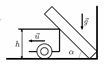
\includegraphics[width = 0.9\textwidth]{0309RotationKinematicsLorry.jpg}
\end{minipage}
\begin{ans}
$\omega = u \sin^2 \alpha /h$
\end{ans}
\end{ex}

\begin{ex}
За лисой, бегущей прямолинейно с постоянной скоростью $v$, бежит собака таким образом, что ее скорость $u$ всегда направлена на местоположение лисы. В момент, когда векторы скоростей перпендикулярны, расстояние между ними было равно $L$. С каким ускорением при этом двигалась собака?
\begin{ans}
$a = uv/L$
\end{ans}
\end{ex}

\begin{ex} 
\hspace{0pt} \\
\begin{minipage}{.65\textwidth}
На диск радиуса $R$ намотаны две нерастяжимые нити, закрепленные в двух разных точках. При отпускании диск вращается. Когда угол между нитями у диска $\alpha$, угловая скорость вращения диска $\omega$. С какой скоростью в этот момент движется центр диска? Нити остаются натянутыми.
\end{minipage}
\begin{minipage}{.35\textwidth}
\centering
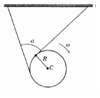
\includegraphics{0311RotationKinematicsDisc.jpg}
\end{minipage}
\begin{ans}
$\omega R/ \cos (\alpha /2)$
\end{ans}
\end{ex}

\begin{ex}
Внутри неподвижной окружности катится без скольжения другая окружность вдвое меньшего радиуса. Какую траекторию описывает при этом произвольно выбранная точка на подвижной окружности?
\begin{ans}
отрезок
\end{ans}
\end{ex}

\begin{ex}
\hspace{0pt} \\
\begin{minipage}{.65\textwidth}
Бусинка может двигаться по кольцу радиуса $R$, подталкиваемая спицей, которая вращается с угловой скоростью $\omega$ в плоскости кольца. Ось вращения спицы находится на кольце. Определить ускорение бусинки.
\end{minipage}
\begin{minipage}{.35\textwidth}
\centering
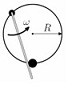
\includegraphics{0313RotationKinematicsRingAndBead.jpg}
\end{minipage}
\begin{ans}
$4 \omega^2 R$
\end{ans}
\end{ex}

\begin{ex}
По палочке, которая вращается с угловой скоростью $\omega$, ползет жук со скоростью $v$. Определите скорость и ускорение жука, когда он находится на расстоянии $L$ от оси вращения палочки.
\begin{ans}
$u = \sqrt{v^2 + \omega^2 L^2}$, $a = \sqrt{\omega^4 L^2 + 4\omega^2 v^2}$
\end{ans}
\end{ex}

\begin{ex}
(2003) Четыре черепахи находятся в вершинах квадрата со стороной $l$. Они начинают двигаться одновременно с постоянной скоростью $v$. Каждая черепаха движется по направлению к своей соседке по часовой стрелке. Где встретятся черепахи и через какое время? Найти угол между скоростью движения черепахи и одной из сторон квадрата как функцию ее координат $\varphi = \varphi (x,y)$.
\begin{ans}
В центре через $t = v/l$, $\tan \alpha = (x-y)/(x+y)$.
\end{ans}
\end{ex}